\documentclass{article}

\usepackage[margin=1in]{geometry}
\usepackage[utf8]{inputenc}
\usepackage[T1]{fontenc}
\usepackage{hyperref}
\usepackage{url}
\usepackage{booktabs}
\usepackage{amsfonts}
\usepackage{nicefrac}
\usepackage{microtype}
\usepackage{xcolor}
\usepackage{graphicx}
\usepackage{float}

\title{Telecom Customer Churn Analysis and Prediction}

\author{%
  Shruti Shukla \\
  Department of Computer Science \\
  Rutgers University \\
  \texttt{scs250@rutgers.edu}
}

\begin{document}

\maketitle

% ── ABSTRACT ──────────────────────────────────────────────────
\begin{abstract}
Customer churn poses a significant challenge in the telecommunications
industry, where acquiring a new customer is substantially more expensive than
retaining an existing one. This project presents an end-to-end machine
learning pipeline for churn prediction using the IBM Telco Customer Churn
dataset (7,032 records). We perform comprehensive data preprocessing,
exploratory data analysis, and feature engineering, then train and evaluate
three classification models: Logistic Regression, Decision Tree, and Random
Forest. Class imbalance is addressed using SMOTE. All models are evaluated
using accuracy, precision, recall, F1-score, and ROC-AUC, with recall
emphasized as the primary metric. Results show that Logistic Regression and
Random Forest achieve AUC $\approx 0.817$, with churn recall of 64\% and
65\% respectively. Feature importance analysis consistently identifies payment
method, tenure, contract type, and monthly charges as the strongest
predictors of churn.
\end{abstract}


% ── 1. INTRODUCTION ───────────────────────────────────────────
\section{Introduction}

Customer churn---the rate at which customers stop doing business with a
company---is a critical metric in subscription-based industries. In
telecommunications, switching costs are low and competition is high, making
retention a constant challenge. Retaining existing customers is generally more cost-effective than acquiring new customers. 

This project investigates the following research question:

\begin{quote}
\textit{Which customer features are most associated with telecom customer
churn, and how effectively can machine learning models predict which customers
are likely to leave?}
\end{quote}

We address this through a full data science pipeline: preprocessing,
exploratory data analysis (EDA), feature engineering, model training, and
evaluation. Beyond predictive accuracy, we emphasize interpretability:
understanding \emph{why} customers churn is as important as predicting
\emph{whether} they will.

\subsection{Prior Work}

Churn prediction has been studied extensively across telecom, e-commerce, and
banking. Standard approaches compare Logistic Regression, Decision Trees, and Random Forest on the same Telco dataset used here. A consistent finding is that contract type, monthly charges, and
tenure are the strongest predictors, which our results confirm. A central
challenge is class imbalance: churners typically represent 20--30\% of
customers. SMOTE [2] is widely used to address this, and we adopt it here.


% ── 2. DATA AND PREPROCESSING ─────────────────────────────────
\section{Data and Preprocessing}

\subsection{Dataset}

We use the IBM Telco Customer Churn dataset [1], sourced from Kaggle. The
dataset contains 7,043 customer records across 21 features, including
demographic information (gender, age, partner, dependents), service
subscriptions (phone, internet, streaming, security), billing details
(contract type, payment method, monthly and total charges), and a binary
churn label. After removing 11 rows with missing \texttt{TotalCharges}
values, the working dataset contains \textbf{7,032 records}.

\subsection{Preprocessing Pipeline}

\paragraph{Feature removal.}
\texttt{customerID} is a unique identifier with no predictive value and was
dropped.

\paragraph{Type conversion.}
\texttt{TotalCharges} was stored as a string in the raw CSV; it was coerced
to numeric and the 11 resulting \texttt{NaN} rows were dropped.

\paragraph{Binary encoding.}
Columns with two categories (gender, Partner, Dependents, PhoneService,
PaperlessBilling, Churn) were mapped to 0/1.

\paragraph{Internet-service encoding.}
Internet-related service columns (OnlineSecurity, OnlineBackup,
DeviceProtection, TechSupport, StreamingTV, StreamingMovies, MultipleLines,
InternetService) were mapped such that any active service becomes 1, while
\texttt{No internet service} and \texttt{No phone service} become 0.

\paragraph{One-hot encoding.}
Contract (three values) and PaymentMethod (four values) were one-hot encoded,
producing six binary dummy features.

\paragraph{Feature engineering.}
Two derived features were created:
\begin{itemize}
  \item \textbf{totalServices}: count of active service subscriptions per
        customer (range 0--9).
  \item \textbf{riskFlag}: binary indicator set to 1 when
        \texttt{tenure} $<$ 37 months \emph{and}
        \texttt{MonthlyCharges} $>$ \$61, identifying customers who are
        both new and high-paying.
\end{itemize}

\paragraph{Train/test split.}
Data was split 80/20 (5,625 training, 1,407 test) using stratified sampling.
SMOTE was applied \emph{only} to the training set, balancing churn and
non-churn to 50/50 before model fitting.


% ── 3. EXPLORATORY DATA ANALYSIS ──────────────────────────────
\section{Exploratory Data Analysis}

\subsection{Churn Distribution}

The dataset is imbalanced: 26.6\% of customers churned (1,869 records) and
73.4\% stayed (5,163 records), as shown in Figure~\ref{fig:churn_dist}. This
motivates the use of SMOTE and the prioritization of recall over accuracy as
the primary evaluation metric.

\begin{figure}[H]
  \centering
  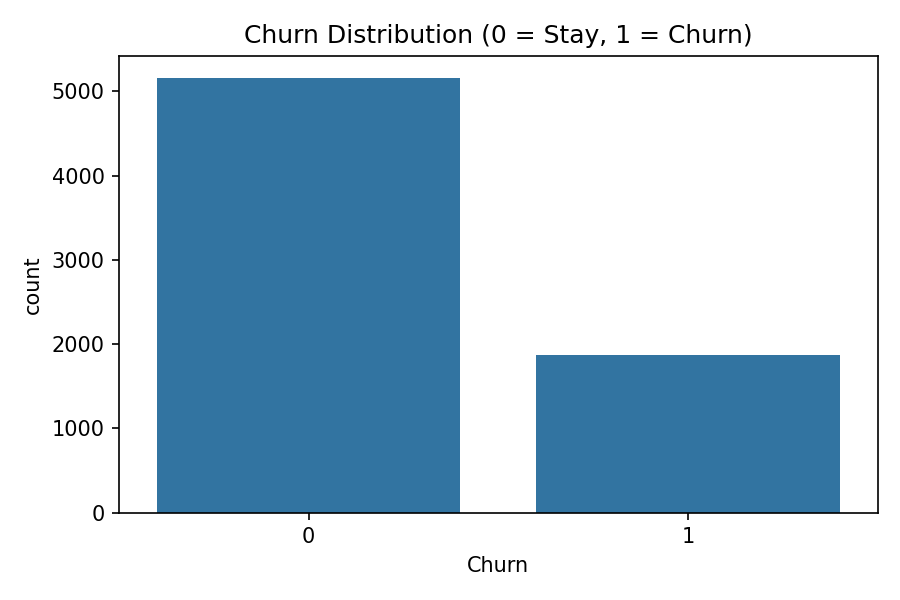
\includegraphics[width=0.45\linewidth]{plot_01_churn_distribution.png}
  \caption{Churn distribution. Approximately 26.6\% of customers churned,
  creating a class imbalance that must be addressed during model training.}
  \label{fig:churn_dist}
\end{figure}

\subsection{Feature Correlations}

Figure~\ref{fig:corr} shows the Pearson correlation of each feature with the
churn label. \textbf{Tenure} has the strongest negative correlation
($r = -0.35$), meaning customers with longer history are substantially less
likely to leave. Internet-related services and \textbf{MonthlyCharges}
show positive correlation with churn, while \textbf{OnlineSecurity}
($r = -0.17$) and \textbf{TechSupport} ($r = -0.16$) show negative
correlation, suggesting that support-related services improve retention.

\begin{figure}[H]
  \centering
  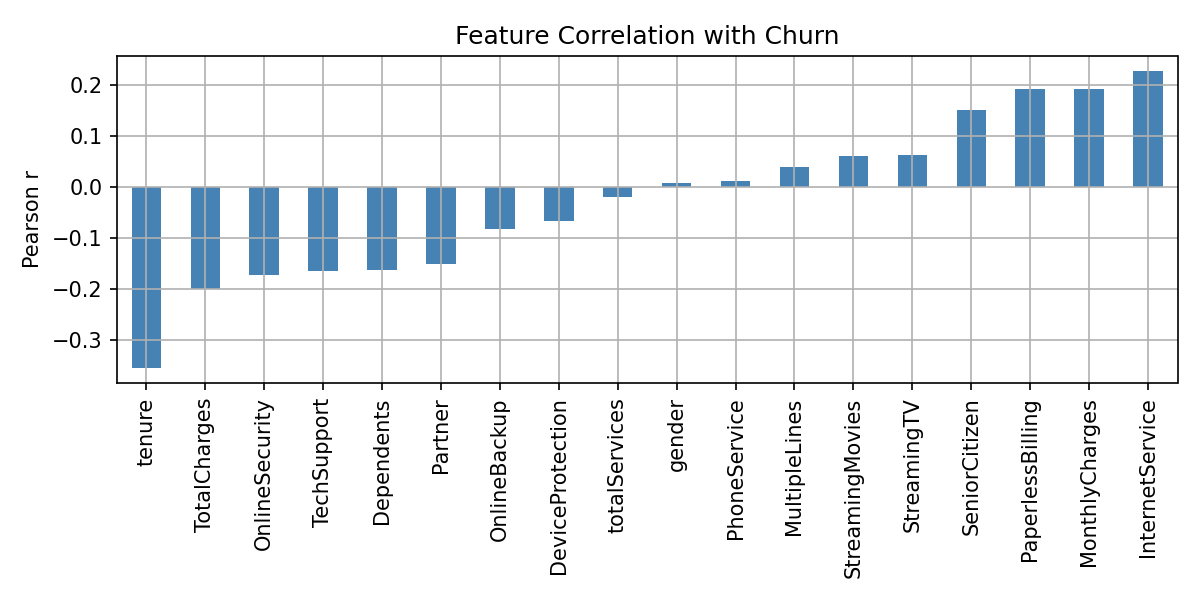
\includegraphics[width=0.85\linewidth]{plot_03_correlation_churn.png}
  \caption{Pearson correlation of each feature with churn. Tenure is the
  strongest negative predictor; InternetService and MonthlyCharges are the
  strongest positive predictors.}
  \label{fig:corr}
\end{figure}

\subsection{Contract Type}

Contract type is the most visually striking predictor
(Figure~\ref{fig:contract}). Month-to-month customers churn at
\textbf{42.7\%}, one-year contract customers at 11.3\%, and two-year contract
customers at just \textbf{2.8\%}. The absence of a long-term commitment
creates a low barrier to switching.

\begin{figure}[H]
  \centering
  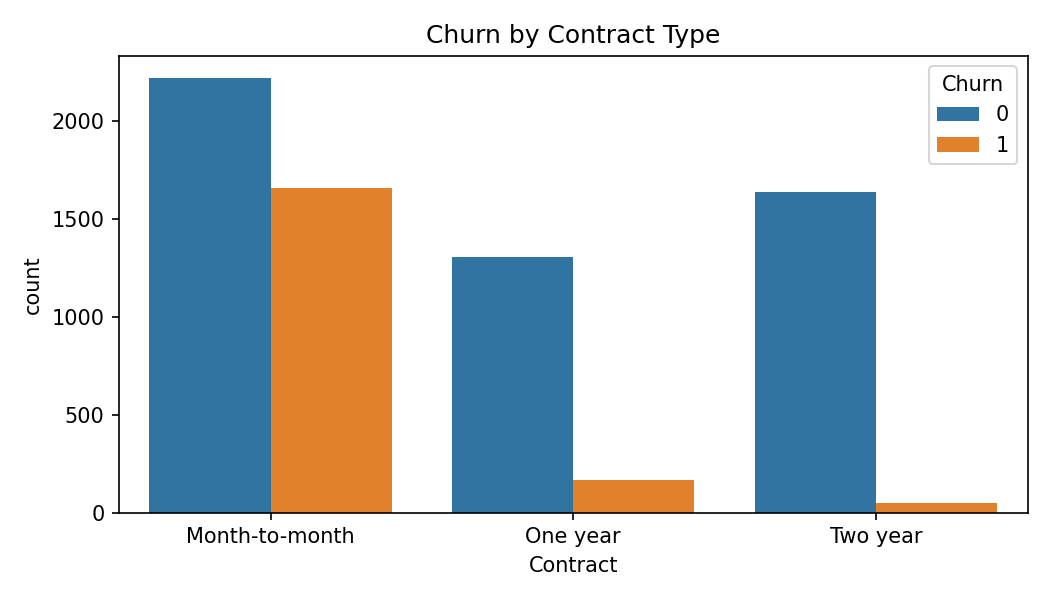
\includegraphics[width=0.6\linewidth]{plot_05_contract_churn.png}
  \caption{Churn counts by contract type. Month-to-month customers account
  for the vast majority of churners; two-year customers almost never leave.}
  \label{fig:contract}
\end{figure}

\subsection{Tenure and Monthly Charges}

Churned customers average \textbf{18.0 months} of tenure, compared to
\textbf{37.7 months} for customers who stayed (Figure~\ref{fig:tenure}).
The scatter plot in Figure~\ref{fig:scatter} shows that churners concentrate
in the upper-left quadrant---short tenure combined with high monthly
charges---which motivates the \textbf{riskFlag} feature. Among high-risk
customers (riskFlag = 1), the churn rate is \textbf{51.3\%}, versus only
16.2\% for the rest.

\begin{figure}[H]
  \centering
  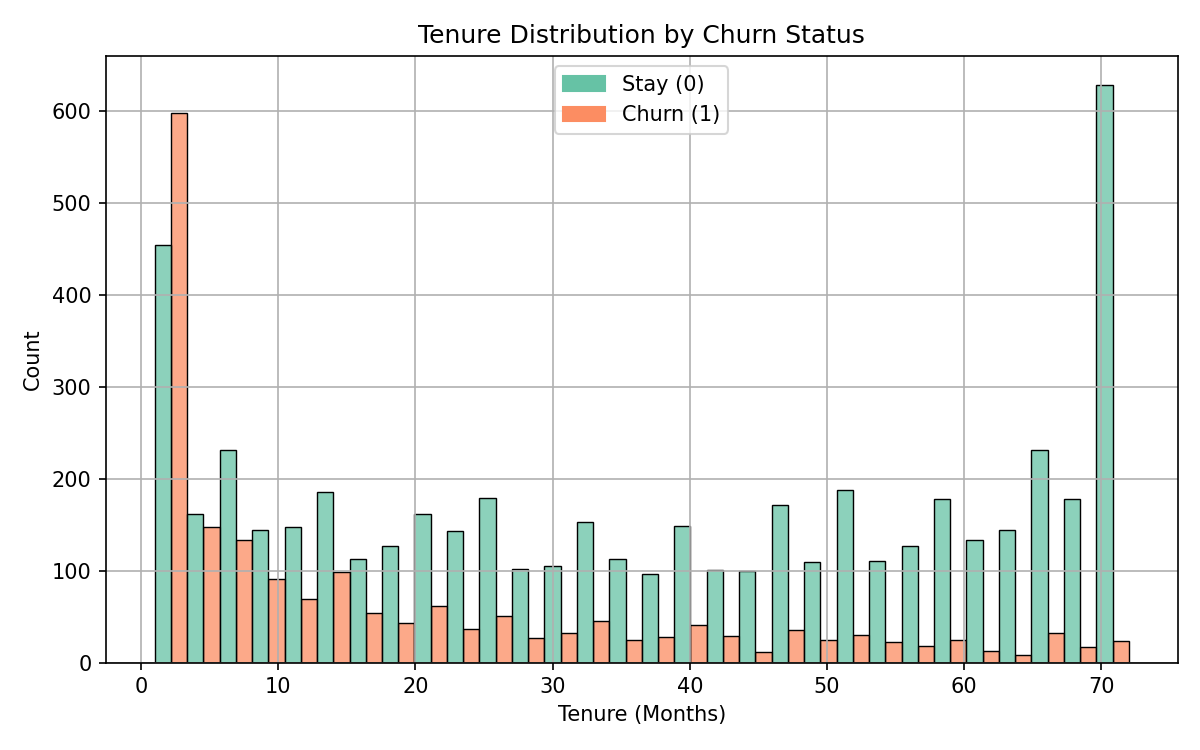
\includegraphics[width=0.75\linewidth]{plot_06_tenure_churn.png}
  \caption{Tenure distribution by churn status. Churners spike in the first
  1--5 months; loyal customers accumulate at 60--72 months.}
  \label{fig:tenure}
\end{figure}

\begin{figure}[H]
  \centering
  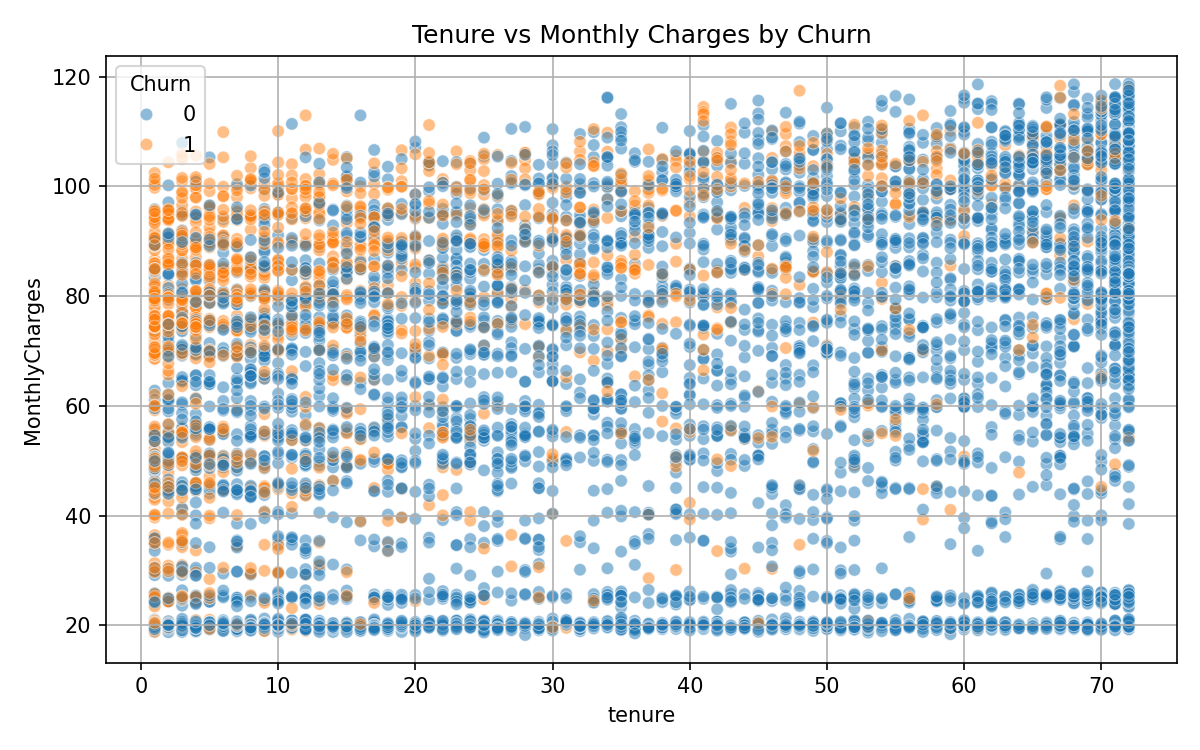
\includegraphics[width=0.75\linewidth]{plot_07_tenure_vs_charges.png}
  \caption{Tenure vs.\ Monthly Charges colored by churn. Churners cluster
  in the high-charge, short-tenure region, validating the riskFlag feature.}
  \label{fig:scatter}
\end{figure}

\subsection{Correlation Heatmap}

Figure~\ref{fig:heatmap} confirms expected multicollinearity: TotalCharges
is highly correlated with both tenure (0.83) and MonthlyCharges (0.65).
The engineered riskFlag correlates with Churn at $r = 0.36$, making it the
second-strongest numerical predictor after tenure.

\begin{figure}[H]
  \centering
  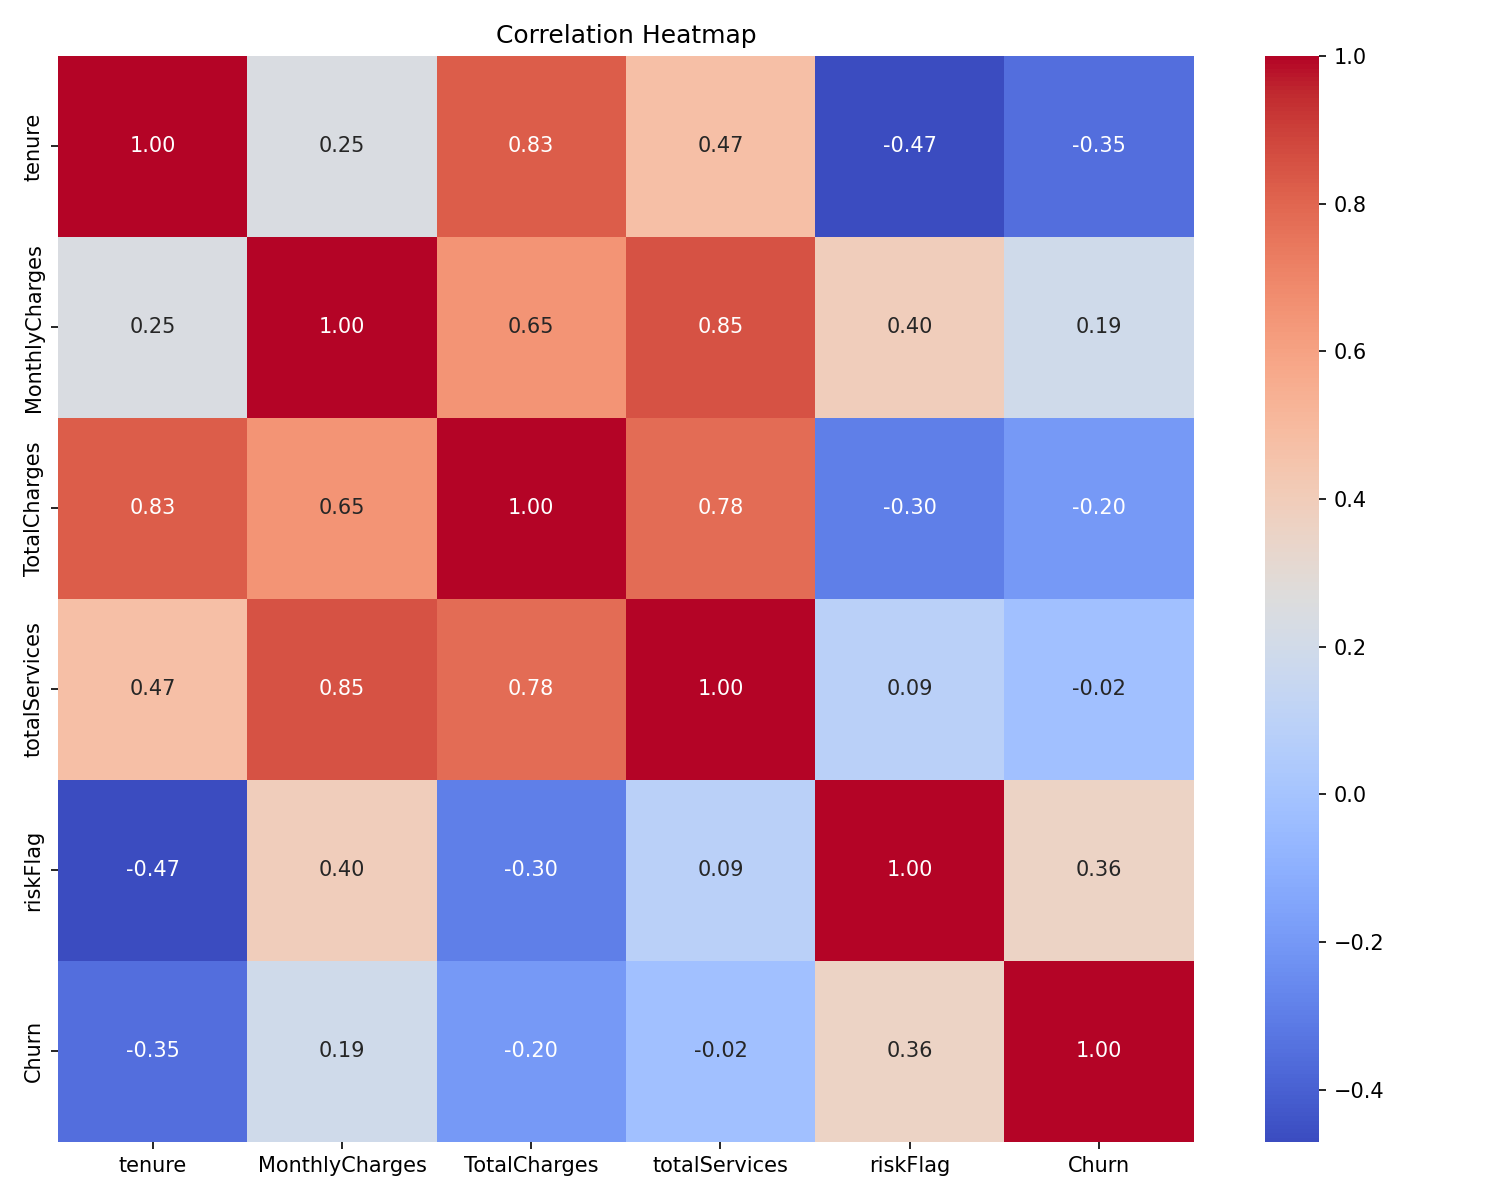
\includegraphics[width=0.65\linewidth]{plot_08_heatmap.png}
  \caption{Correlation heatmap of numerical features. The strong
  TotalCharges--tenure correlation (0.83) reflects its composite nature.
  riskFlag achieves $r = 0.36$ with Churn.}
  \label{fig:heatmap}
\end{figure}


% ── 4. METHODOLOGY ────────────────────────────────────────────
\section{Methodology}

\subsection{Models}

Three classifiers were selected to span the complexity--interpretability
tradeoff:

\paragraph{Logistic Regression.}
Used as the interpretable baseline. Churn probability is estimated via:
\[
  P(Y=1 \mid \mathbf{x})
  = \frac{1}{1 + e^{-(\alpha + \boldsymbol{\beta}^\top \mathbf{x})}}.
\]
Parameters were estimated by maximum likelihood with \texttt{max\_iter=3000}.
Coefficients provide direct insight into each feature's directional effect on
churn probability.

\paragraph{Decision Tree.}
Trained with \texttt{max\_depth=6} to prevent overfitting. Splits maximize
information gain. The resulting tree is interpretable as a set of
human-readable rules; feature importances reflect aggregate impurity
reduction.

\paragraph{Random Forest.}
An ensemble of 100 decision trees (\texttt{max\_depth=10}) [3], each trained
on a random feature and sample subset. Averaging predictions across trees
reduces variance and improves generalization. Feature importances are averaged
across all trees.

\subsection{Evaluation Metrics}

Accuracy alone is insufficient under class imbalance. We report:
\begin{itemize}
  \item \textbf{Recall} (primary): fraction of actual churners correctly
        identified. Missing a churner is costly---the customer is lost
        entirely.
  \item \textbf{Precision}: fraction of predicted churners who actually
        churned. Low precision wastes retention resources.
  \item \textbf{F1-score}: harmonic mean of precision and recall.
  \item \textbf{ROC-AUC}: discriminative ability across all classification
        thresholds.
  \item \textbf{Confusion matrix}: breakdown of true/false positives and
        negatives.
\end{itemize}


% ── 5. RESULTS ────────────────────────────────────────────────
\section{Results}

\subsection{Model Performance}

Table~\ref{tab:results} summarizes performance on the held-out test set
(1,407 samples). All three models achieve similar accuracy (74--76\%);
differences emerge most clearly in recall and ROC-AUC.

\begin{table}[H]
  \caption{Model performance on the test set (1,407 samples). Recall is the
  primary metric. Logistic Regression achieves the best balance of recall and
  ROC-AUC.}
  \label{tab:results}
  \centering
  \begin{tabular}{lccccc}
    \toprule
    Model & Accuracy & Precision & Recall & F1 & ROC-AUC \\
    \midrule
    Logistic Regression & 0.760 & 0.54 & 0.64 & 0.59 & \textbf{0.817} \\
    Decision Tree       & 0.740 & 0.52 & \textbf{0.66} & 0.58 & 0.785 \\
    Random Forest       & 0.750 & 0.53 & 0.65 & 0.58 & 0.816 \\
    \bottomrule
  \end{tabular}
\end{table}

\subsection{ROC-AUC Curves}

Figure~\ref{fig:roc} shows ROC curves for all three models. Logistic
Regression (AUC = 0.817) and Random Forest (AUC = 0.816) are nearly
indistinguishable, both well above the diagonal. The Decision Tree
(AUC = 0.785) trails slightly---a typical result, since individual trees are
more sensitive to training-data variance than ensembles.

\begin{figure}[H]
  \centering
  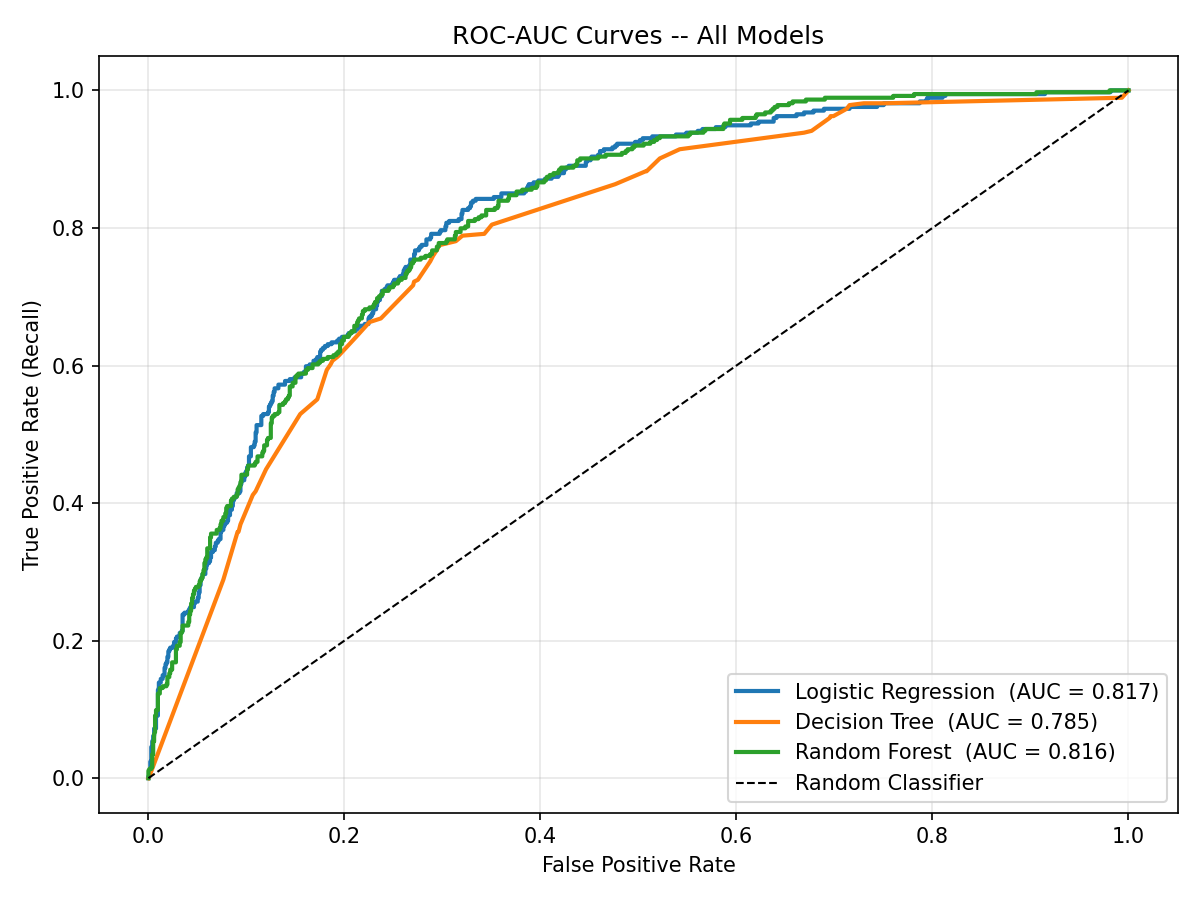
\includegraphics[width=0.7\linewidth]{plot_09_roc_auc.png}
  \caption{ROC-AUC curves for all three models. Logistic Regression and
  Random Forest achieve near-identical AUC of 0.817 and 0.816, both
  substantially above the random baseline.}
  \label{fig:roc}
\end{figure}

\subsection{Confusion Matrices}

Figure~\ref{fig:cm} shows confusion matrices on the test set. Of 374 true
churners: Logistic Regression correctly identifies 239, Decision Tree 248,
and Random Forest 243. However, the Decision Tree also produces the most
false positives (233), while Logistic Regression produces the fewest (203).
This trade-off has a direct business interpretation: if the goal is to catch
as many churners as possible, the Decision Tree wins on recall; if the goal
is efficient targeting of retention resources, Logistic Regression's lower
false-positive rate is preferable.

\begin{figure}[H]
  \centering
  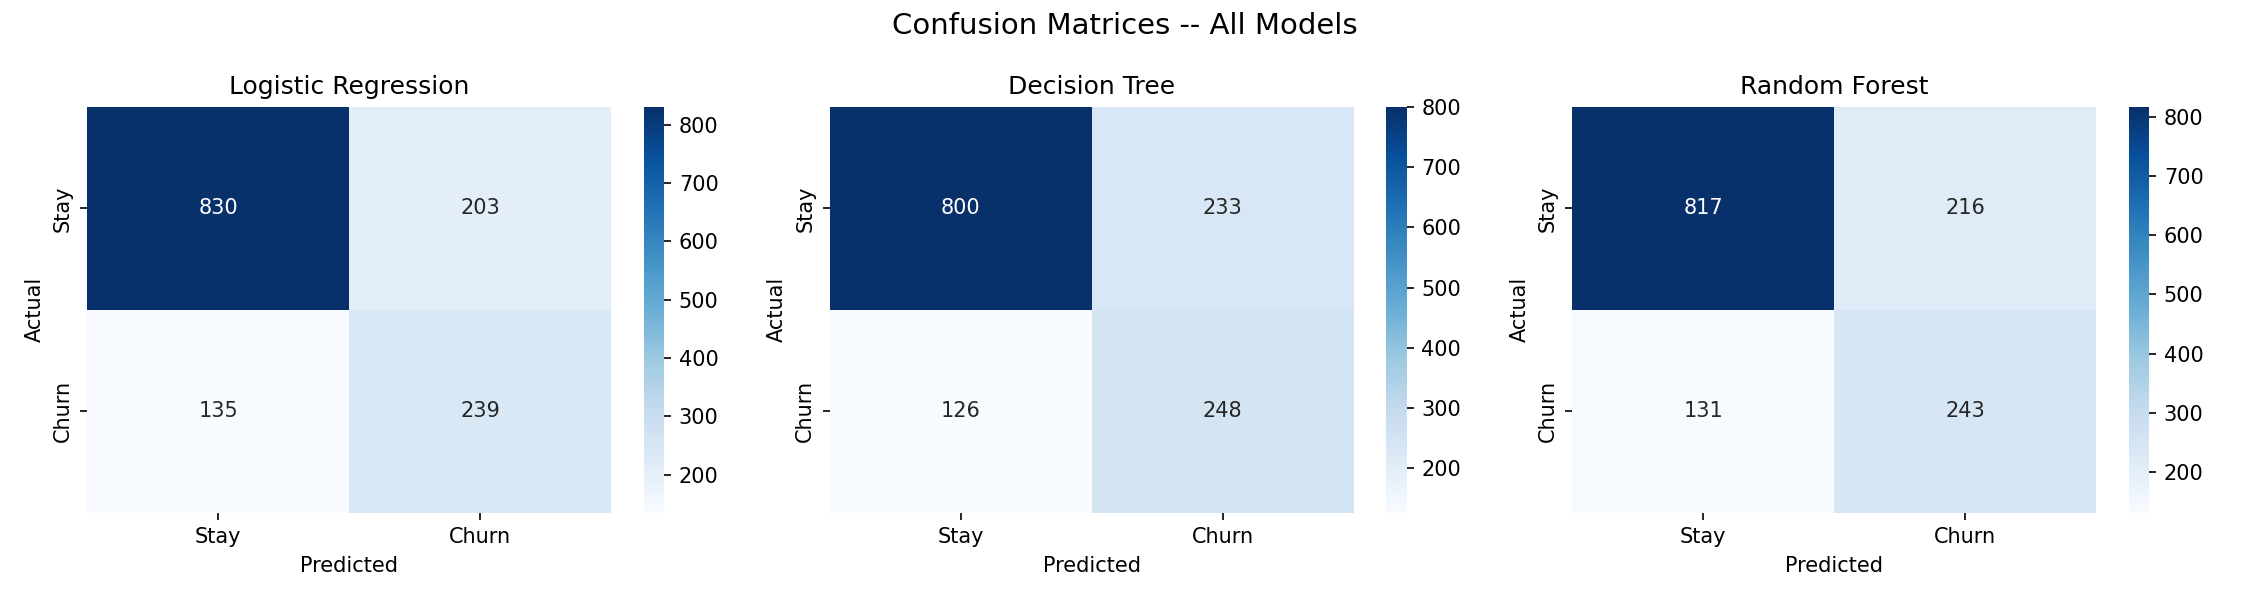
\includegraphics[width=\linewidth]{plot_10_confusion_matrices.png}
  \caption{Confusion matrices for all three models. Decision Tree catches the
  most churners (248) at the cost of the most false positives (233). Logistic
  Regression offers the best precision--recall balance.}
  \label{fig:cm}
\end{figure}

\subsection{Feature Importance}

Figure~\ref{fig:fi} shows feature importances across all three models. Key
findings:

\begin{itemize}
  \item \textbf{PaymentMethod\_Electronic check} consistently appears among the strongest predictors
across all models, with importance 0.44 in Decision Tree and 0.15 in Random Forest, and
        shows a large positive coefficient in Logistic Regression. Customers
        paying by electronic check churn at a higher rate, possibly reflecting
        lower engagement or fewer automatic payment commitments.
  \item \textbf{Tenure} is the dominant predictor by Logistic Regression
        coefficient magnitude (most negative: longer tenure strongly predicts
        staying) and ranks second in Random Forest.
  \item \textbf{MonthlyCharges} ranks third in Random Forest, consistent with
        its positive EDA correlation with churn.
  \item \textbf{Contract type} (two-year, one-year) ranks in the top features
        of all three models, confirming that contractual commitment is a
        primary retention mechanism.
  \item \textbf{OnlineSecurity} and \textbf{TechSupport} rank highly in
        Logistic Regression and Random Forest, suggesting that value-added
        services reduce churn risk.
\end{itemize}

\begin{figure}[H]
  \centering
  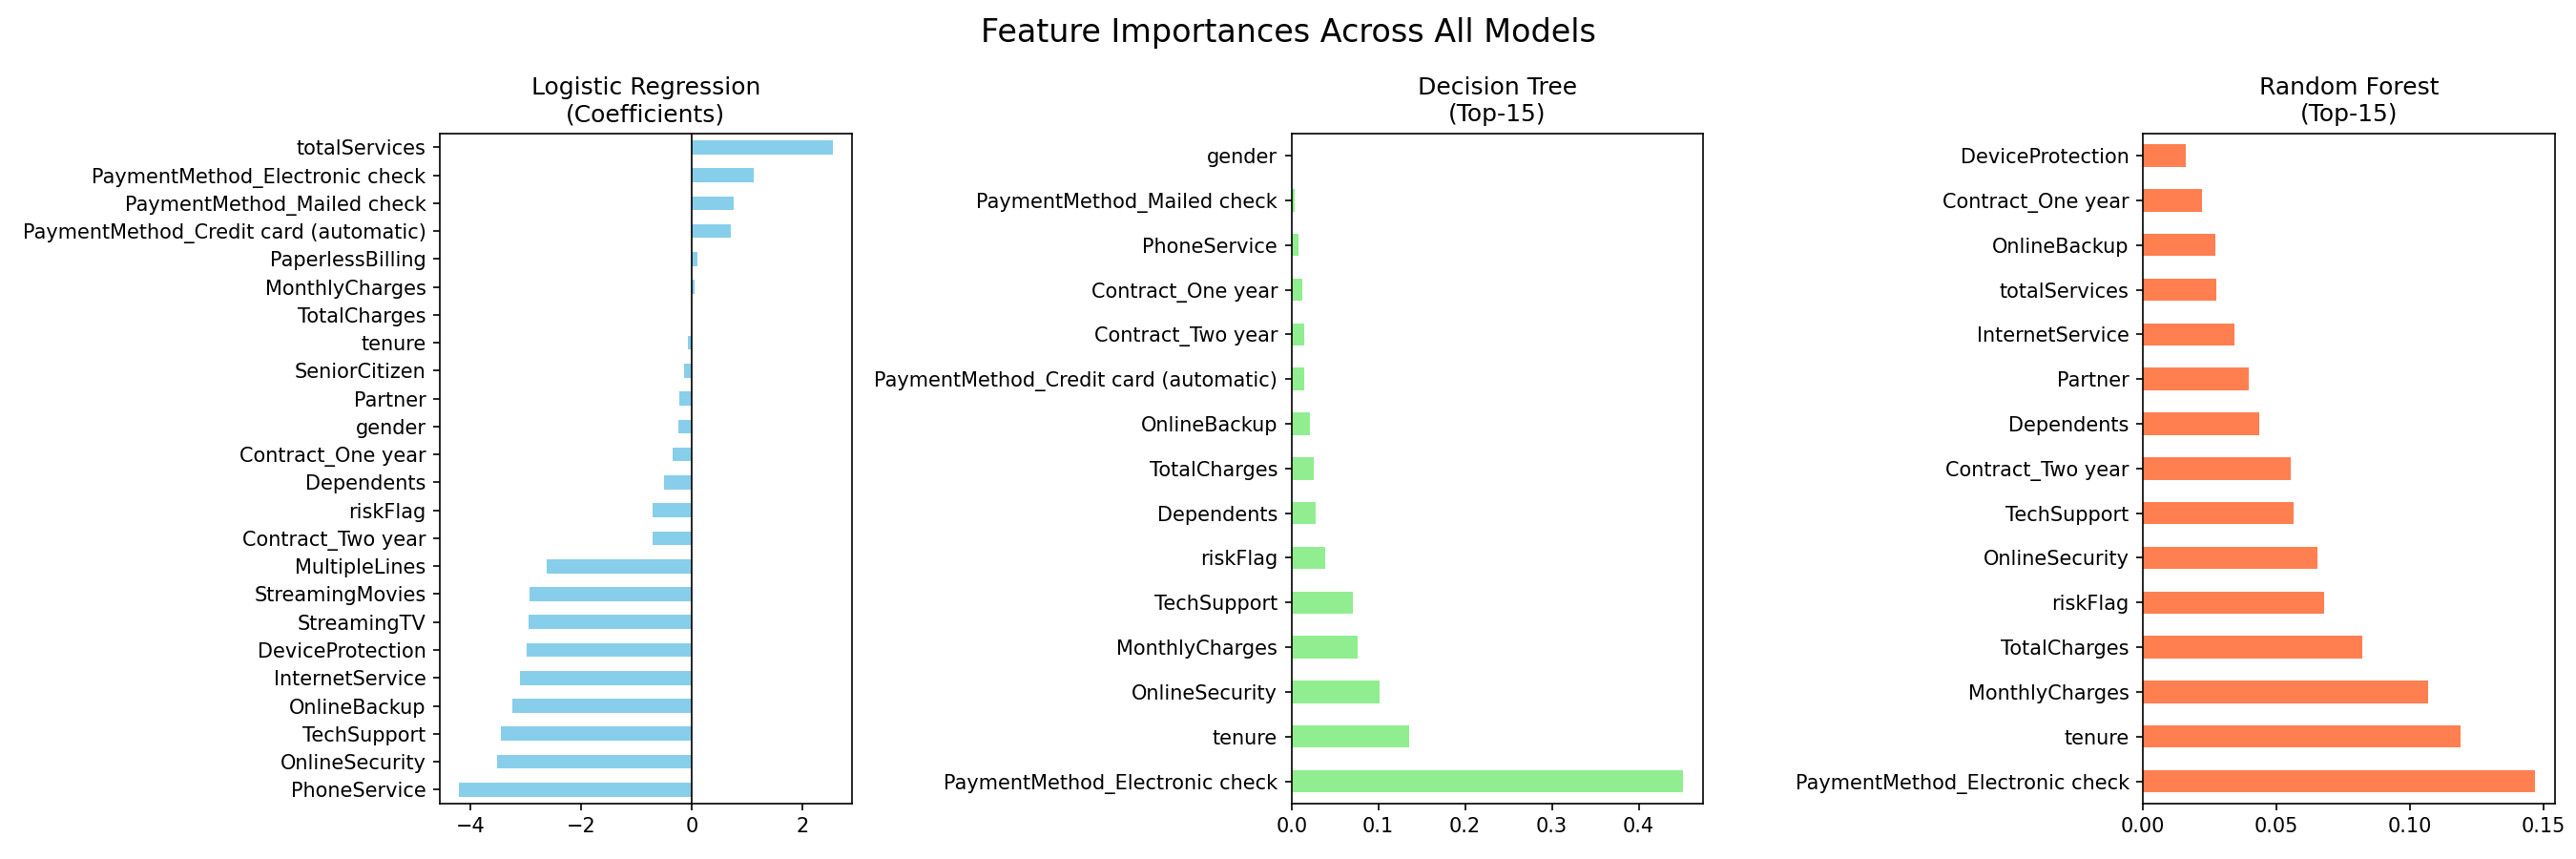
\includegraphics[width=\linewidth]{plot_11_feature_importance.png}
  \caption{Feature importances across all three models. Despite different
  algorithms, all three consistently identify payment method, tenure, and
  contract type as dominant predictors.}
  \label{fig:fi}
\end{figure}


% ── 6. DISCUSSION ─────────────────────────────────────────────
\section{Discussion}

The results provide insight into the research question. The features most
associated with churn are: (1)~electronic check payment, (2)~short tenure,
(3)~month-to-month contract, (4)~high monthly charges, and (5)~absence of
security or support add-ons. This profile describes a customer who is new,
pays a premium, has no long-term commitment, and lacks additional support or security-related services---more likely to churn based on observed patterns.

All three models achieve AUC $\approx 0.82$, representing strong lift over
random guessing. 
The engineered \textbf{riskFlag} feature demonstrates that domain-driven
feature engineering can surface high-risk segments without complex modeling.
Its 51.3\% churn rate among flagged customers (vs.\ 16.2\% for others) makes
it useful for identifying high-risk customer groups.

\paragraph{Limitations.}
The dataset covers a single provider, so generalizability to other markets is
not guaranteed. SMOTE was applied before feature importance computation,
meaning importance scores partly reflect the augmented distribution.
No hyperparameter tuning was performed; grid or random search could improve
recall further, particularly for Random Forest.


% ── 7. CONCLUSION ─────────────────────────────────────────────
\section{Conclusion}

This project demonstrated that telecom customer churn can be predicted with
meaningful accuracy using demographic and billing features. Key takeaways:

\begin{itemize}
  \item Tenure, contract type, and payment method are the strongest
        predictors of churn.
  \item Month-to-month customers churn at 42.7\%---fifteen times the rate of
        two-year contract customers (2.8\%).
  \item Logistic Regression achieves AUC = 0.817 and recall = 64\%, matching
        the more complex Random Forest (AUC = 0.816, recall = 65\%).
  \item A simple riskFlag feature identifies a segment churning at 51.3\%.
\end{itemize}

The most actionable recommendation is to prioritize retention outreach toward
month-to-month customers paying by electronic check with tenure under 37
months, particularly those without online security or tech support. Contract
upgrade incentives and bundled service discounts targeted at this segment
could meaningfully reduce churn.

\section*{References}

{
\small

[1] Moro, S.\ (2017). Telco Customer Churn Dataset. \textit{Kaggle}.
\url{https://www.kaggle.com/datasets/blastchar/telco-customer-churn}

[2] Chawla, N.V., Bowyer, K.W., Hall, L.O., \& Kegelmeyer, W.P.\ (2002).
SMOTE: Synthetic minority over-sampling technique. \textit{Journal of
Artificial Intelligence Research}, 16, 321--357.

[3] Breiman, L.\ (2001). Random forests. \textit{Machine Learning},
45(1), 5--32.

[4] Pedregosa, F., et al.\ (2011). Scikit-learn: Machine learning in Python.
\textit{Journal of Machine Learning Research}, 12, 2825--2830.

}

\end{document}
